\documentclass[10pt,twocolumn,letterpaper]{article}

% Packages
\usepackage{times}
\usepackage{epsfig}
\usepackage{graphicx}
\usepackage{amsmath}
\usepackage{amssymb}
\usepackage{booktabs}
\usepackage{algorithm}
\usepackage{algorithmic}
\usepackage{hyperref}
\usepackage[margin=0.75in]{geometry}

% Page setup
\setlength{\columnsep}{0.25in}

\title{\Large \bf Efficient Liveness Detection via Frequency-Decoupled \\ Variational Autoencoder with Landmark-Only Input}

\author{
Anonymous Submission
}

\date{}

\begin{document}

\maketitle
\thispagestyle{empty}

\begin{abstract}
Face liveness detection is critical for preventing presentation attacks in face recognition systems. However, existing methods often require extensive labeled fake samples and computationally expensive deep networks. We propose an efficient two-stage approach combining frequency-decoupled variational autoencoders (VAE) with landmark-only input. Stage 1 performs one-class learning on real samples using a band-split VAE decomposing facial motion into interpretable frequency bands. Stage 2 fine-tunes with minimal fake samples using margin-based or discriminative losses. By operating solely on 40 facial landmarks, our method achieves 89.26\% F1-score with 2.7M parameters—38$\times$ smaller than video-based approaches. The frequency decomposition provides interpretability, revealing characteristic anomalies in different bands for various attack types.
\end{abstract}

\section{Introduction}

Face recognition systems are vulnerable to presentation attacks using photos, videos, or deepfake content. Liveness detection—distinguishing live faces from fake presentations—is essential for biometric security.

Traditional methods rely on hand-crafted features like texture analysis or motion patterns. Recent deep learning approaches achieve higher accuracy but require: (1) extensive labeled datasets of real and fake samples, (2) computationally expensive 3D CNNs processing full video frames, and (3) substantial model parameters.

We identify three fundamental limitations. First, \textbf{data efficiency}: most methods require large-scale fake datasets, expensive to collect and quickly outdated. Second, \textbf{computational efficiency}: processing full frames incurs high costs. Third, \textbf{interpretability}: deep models provide limited insight into classification rationale.

We propose a two-stage framework addressing these through three contributions:

\textbf{(1) Landmark-only representation:} We operate on 40 facial landmark trajectories rather than pixels, reducing dimensionality from $300 \times H \times W \times 3$ to $300 \times 40 \times 2$, achieving $>1000\times$ parameter reduction while preserving motion dynamics.

\textbf{(2) Efficient two-stage learning:} Stage 1 employs one-class learning on real samples only via VAE. Stage 2 fine-tunes with minimal fake samples (538 vs. 1088 real), demonstrating extensive fake datasets are unnecessary.

\textbf{(3) Frequency-decoupled architecture:} We introduce band-split VAE decomposing facial motion into three interpretable bands—low (0-2Hz), band-pass (2-8Hz), high (8-15Hz)—corresponding to head pose, speech motion, and micro-expressions. This enables interpretability and reveals band-specific anomalies in fake videos.

Our experiments show Method 1 (Margin) achieves 88.89\% F1 and Method 2 (Discriminator) reaches 89.26\% F1, significantly outperforming Stage 1 baseline (86.64\%) with only 538 fake samples.

\section{Method}

\subsection{Input Representation}

Given video sequence length $T=300$ frames at 30 fps (10 seconds), we extract 40 facial landmarks per frame. Let $\mathbf{L}_t \in \mathbb{R}^{40 \times 2}$ denote landmarks at frame $t$, normalized by image dimensions. We construct feature tensor $\mathbf{X} \in \mathbb{R}^{T \times 40 \times F}$ where $F=8$ includes:
\begin{itemize}
\itemsep0em
    \item Position: $(x, y)$ coordinates
    \item Velocity: $\mathbf{v}_t = (\mathbf{L}_t - \mathbf{L}_{t-1}) \cdot \text{fps}$
    \item Acceleration: $\mathbf{a}_t = (\mathbf{v}_t - \mathbf{v}_{t-1}) \cdot \text{fps}$
    \item Angle: $\theta_t = \arctan2(y, x)$
    \item Angular velocity: $\dot{\theta}_t = (\theta_t - \theta_{t-1}) \cdot \text{fps}$
\end{itemize}

\subsection{Band-Split VAE Architecture}

We apply 4th-order Butterworth filters decomposing $\mathbf{X}$ into three frequency bands:
\begin{align}
    \mathbf{X}_{\text{LF}} &= \text{LowPass}(\mathbf{X}, f_c=2\text{Hz}) \\
    \mathbf{X}_{\text{BP}} &= \text{BandPass}(\mathbf{X}, [2, 8]\text{Hz}) \\
    \mathbf{X}_{\text{HF}} &= \text{HighPass}(\mathbf{X}, f_c=8\text{Hz})
\end{align}

Figure~\ref{fig:architecture} illustrates the architecture. Each band is processed by an independent VAE with shared architecture.

\begin{figure}[t]
\centering
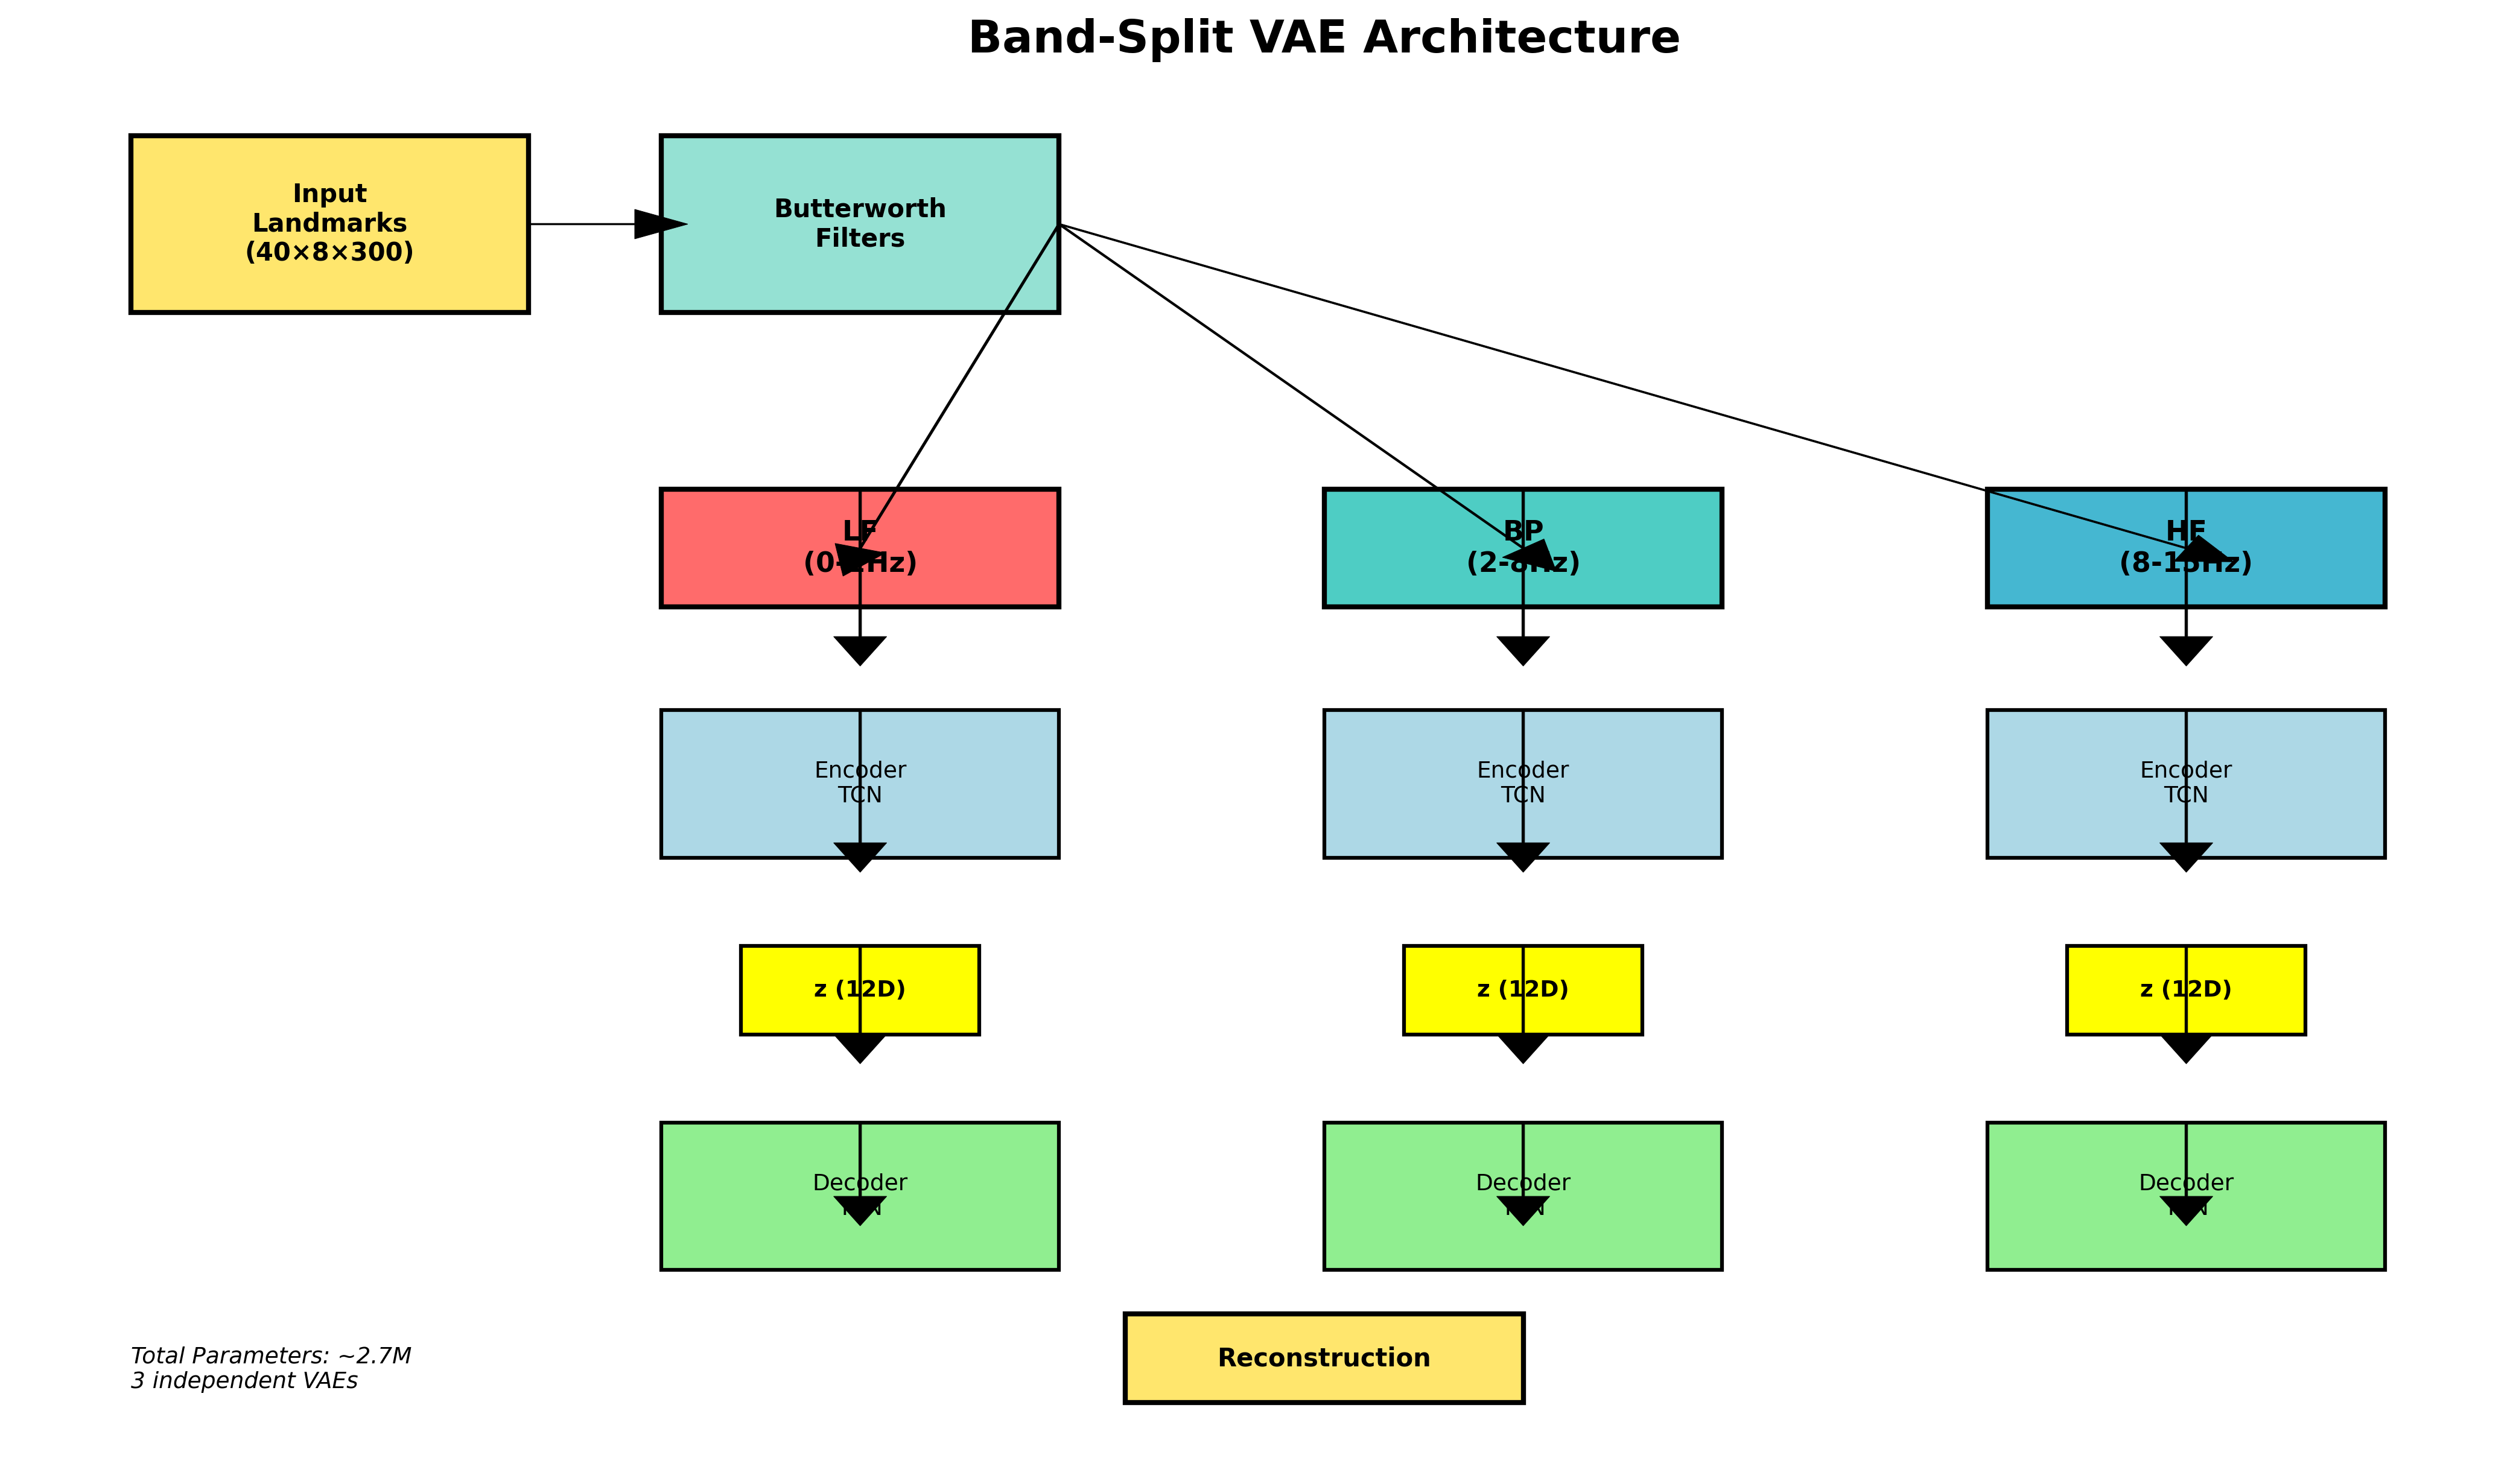
\includegraphics[width=0.48\textwidth]{paper_figures/figure5_architecture.png}
\caption{Band-Split VAE Architecture. Input landmarks decompose into three frequency bands (LF, BP, HF), each processed by independent VAE with shared hyperparameters but separate weights.}
\label{fig:architecture}
\vspace{-1em}
\end{figure}

\textbf{Encoder:} For band $b \in \{\text{LF}, \text{BP}, \text{HF}\}$, encoder maps $\mathbf{X}_b \in \mathbb{R}^{C_{\text{in}} \times T}$ (where $C_{\text{in}} = 320$) to latent parameters:
\begin{align}
    \mathbf{h}_b &= \text{TCN}_{\text{enc}}(\mathbf{X}_b; C_h=48) \\
    [\boldsymbol{\mu}_b, \log\boldsymbol{\sigma}^2_b] &= \text{Conv1D}(\mathbf{h}_b) \in \mathbb{R}^{2C_z \times T}
\end{align}
where TCN uses dilated convolutions $[1,2,4]$, $C_h=48$ hidden channels, $C_z=12$ latent dimensions.

\textbf{Decoder:} Latent codes sampled via reparameterization $\mathbf{z}_b = \boldsymbol{\mu}_b + \boldsymbol{\sigma}_b \odot \boldsymbol{\epsilon}$ where $\boldsymbol{\epsilon} \sim \mathcal{N}(0, \mathbf{I})$:
\begin{equation}
    \hat{\mathbf{X}}_b = \text{TCN}_{\text{dec}}(\mathbf{z}_b; C_h=48)
\end{equation}

The model has three independent VAEs totaling $\sim$2.7M parameters (vs. $>$100M for video-based 3D CNNs).

\subsection{Stage 1: One-Class Pretraining}

Stage 1 trains exclusively on real samples $\{\mathbf{X}^{(i)}_{\text{real}}\}_{i=1}^{N_{\text{real}}}$ with VAE loss:
\begin{equation}
\mathcal{L}_{\text{VAE}} = \sum_{b} \left[ \|\mathbf{X}_b - \hat{\mathbf{X}}_b\|_1 + \beta D_{\text{KL}}(\mathcal{N}(\boldsymbol{\mu}_b, \boldsymbol{\sigma}^2_b) \| \mathcal{N}(0, \mathbf{I})) \right]
\end{equation}
where $\beta=1.0$ and $D_{\text{KL}}$ denotes KL divergence. L1 loss is robust to outliers.

This learns the manifold of genuine facial motion. Real samples exhibit: (i) LF band: smooth head pose, (ii) BP band: periodic speech motion, (iii) HF band: natural micro-expressions. Fake videos deviate, enabling anomaly detection.

\subsection{Stage 2: Discriminative Fine-tuning}

Stage 2 introduces fake samples $\{\mathbf{X}^{(j)}_{\text{fake}}\}_{j=1}^{N_{\text{fake}}}$ where $N_{\text{fake}} = 538 \ll N_{\text{real}} = 1088$.

\textbf{Method 1 (Margin):} Encourage fake samples' reconstruction loss above margin $m$:
\begin{equation}
\mathcal{L}_{\text{margin}} = \mathbb{E}_{\mathbf{X}_{\text{real}}}[\mathcal{L}_{\text{VAE}}] + \mathbb{E}_{\mathbf{X}_{\text{fake}}}[\max(0, m - \mathcal{L}_{\text{VAE}})]
\end{equation}
where $m=0.5$. This pushes fakes from real manifold.

\textbf{Method 2 (Discriminator):} Add discriminator $D_\phi$ on concatenated latents:
\begin{align}
    \mathbf{z}_{\text{concat}} &= [\text{pool}(\boldsymbol{\mu}_{\text{LF}}); \text{pool}(\boldsymbol{\mu}_{\text{BP}}); \text{pool}(\boldsymbol{\mu}_{\text{HF}})] \\
    \text{pool}(\boldsymbol{\mu}) &= [\text{mean}(\boldsymbol{\mu}); \max(\boldsymbol{\mu})] \in \mathbb{R}^{2C_z}
\end{align}

Discriminator is 3-layer MLP with 128 hidden units. Total loss:
\begin{equation}
\mathcal{L}_{\text{total}} = \mathcal{L}_{\text{VAE}} + \lambda \mathcal{L}_{\text{BCE}}(D_\phi(\mathbf{z}), y)
\end{equation}
where $\lambda=1.0$.

\subsection{Inference: Two-Stage Gaussian Filtering}

We use statistical approach based on Gaussian modeling of real samples.

\textbf{Stage 1 Filter:} Compute reconstruction loss per band:
\begin{equation}
\ell_b = \|\mathbf{X}_b - \hat{\mathbf{X}}_b\|_2^2, \quad b \in \{\text{LF, BP, HF}\}
\end{equation}

Form 3D vector $\mathbf{\ell} = [\ell_{\text{LF}}, \ell_{\text{BP}}, \ell_{\text{HF}}]^\top$ and fit $\mathcal{N}(\boldsymbol{\mu}_\ell, \boldsymbol{\Sigma}_\ell)$ on real training samples. Test sample passes if:
\begin{equation}
(\mathbf{\ell} - \boldsymbol{\mu}_\ell)^\top \boldsymbol{\Sigma}_\ell^{-1} (\mathbf{\ell} - \boldsymbol{\mu}_\ell) \leq \chi^2_{0.95}(3)
\end{equation}

\textbf{Stage 2 Filter:} Extract latent vectors by temporal averaging, apply PCA to 10D (preserving $>91\%$ variance), fit $\mathcal{N}(\boldsymbol{\mu}_z, \boldsymbol{\Sigma}_z)$ on real samples. Classify as real only if both filters pass:
\begin{equation}
\text{Prediction} = \begin{cases}
\text{Real} & \text{if both pass} \\
\text{Fake} & \text{otherwise}
\end{cases}
\end{equation}

\section{Experiments}

\subsection{Dataset and Setup}

Our dataset consists of two distinct sources:

\textbf{Stage 1 Training (Real only):} We use a large-scale real video dataset from \texttt{20GBprocessed/} directory containing authentic facial videos captured in natural conditions. From this, we randomly sample 1088 real videos for Stage 1 one-class VAE pretraining. These videos represent genuine facial motion across diverse subjects and conditions.

\textbf{Stage 2 Training (Real + Fake):} For Stage 2 fine-tuning, we combine:
\begin{itemize}
\itemsep0em
    \item Same 1088 real samples from Stage 1
    \item 538 fake samples: balanced mix of replay attacks (phone-replayed videos) and audio-driven deepfakes
\end{itemize}

\textbf{Testing:} 117 real, 117 fake (balanced, held-out set, disjoint from training).

All videos are 10 seconds at 30 fps. We extract 40 facial landmarks (20 outer lip, 20 inner lip contour) per frame using pre-trained detector.

Training uses Adam optimizer ($\text{lr}=10^{-4}$), batch size 64, 20 epochs (Stage 1), 10 epochs (Stage 2), mixed precision on single GPU.

\subsection{Main Results}

Table~\ref{tab:main_results} compares three models on 234-sample test set.

\begin{table}[h]
\caption{Performance on test set. All use two-stage Gaussian filtering.}
\label{tab:main_results}
\centering
\small
\begin{tabular}{lccccc}
\toprule
Method & Acc & Prec & Rec & F1 & Spec \\
\midrule
Stage 1 & 85.90 & 82.31 & 91.45 & 86.64 & 80.34 \\
Method 1 & 88.46 & 85.71 & 92.31 & 88.89 & 84.62 \\
Method 2 & \bf 88.89 & \bf 86.40 & \bf 92.31 & \bf 89.26 & \bf 85.47 \\
\bottomrule
\end{tabular}
\vspace{-0.5em}
\end{table}

Figure~\ref{fig:main_results} visualizes performance across metrics.

\begin{figure}[t]
\centering
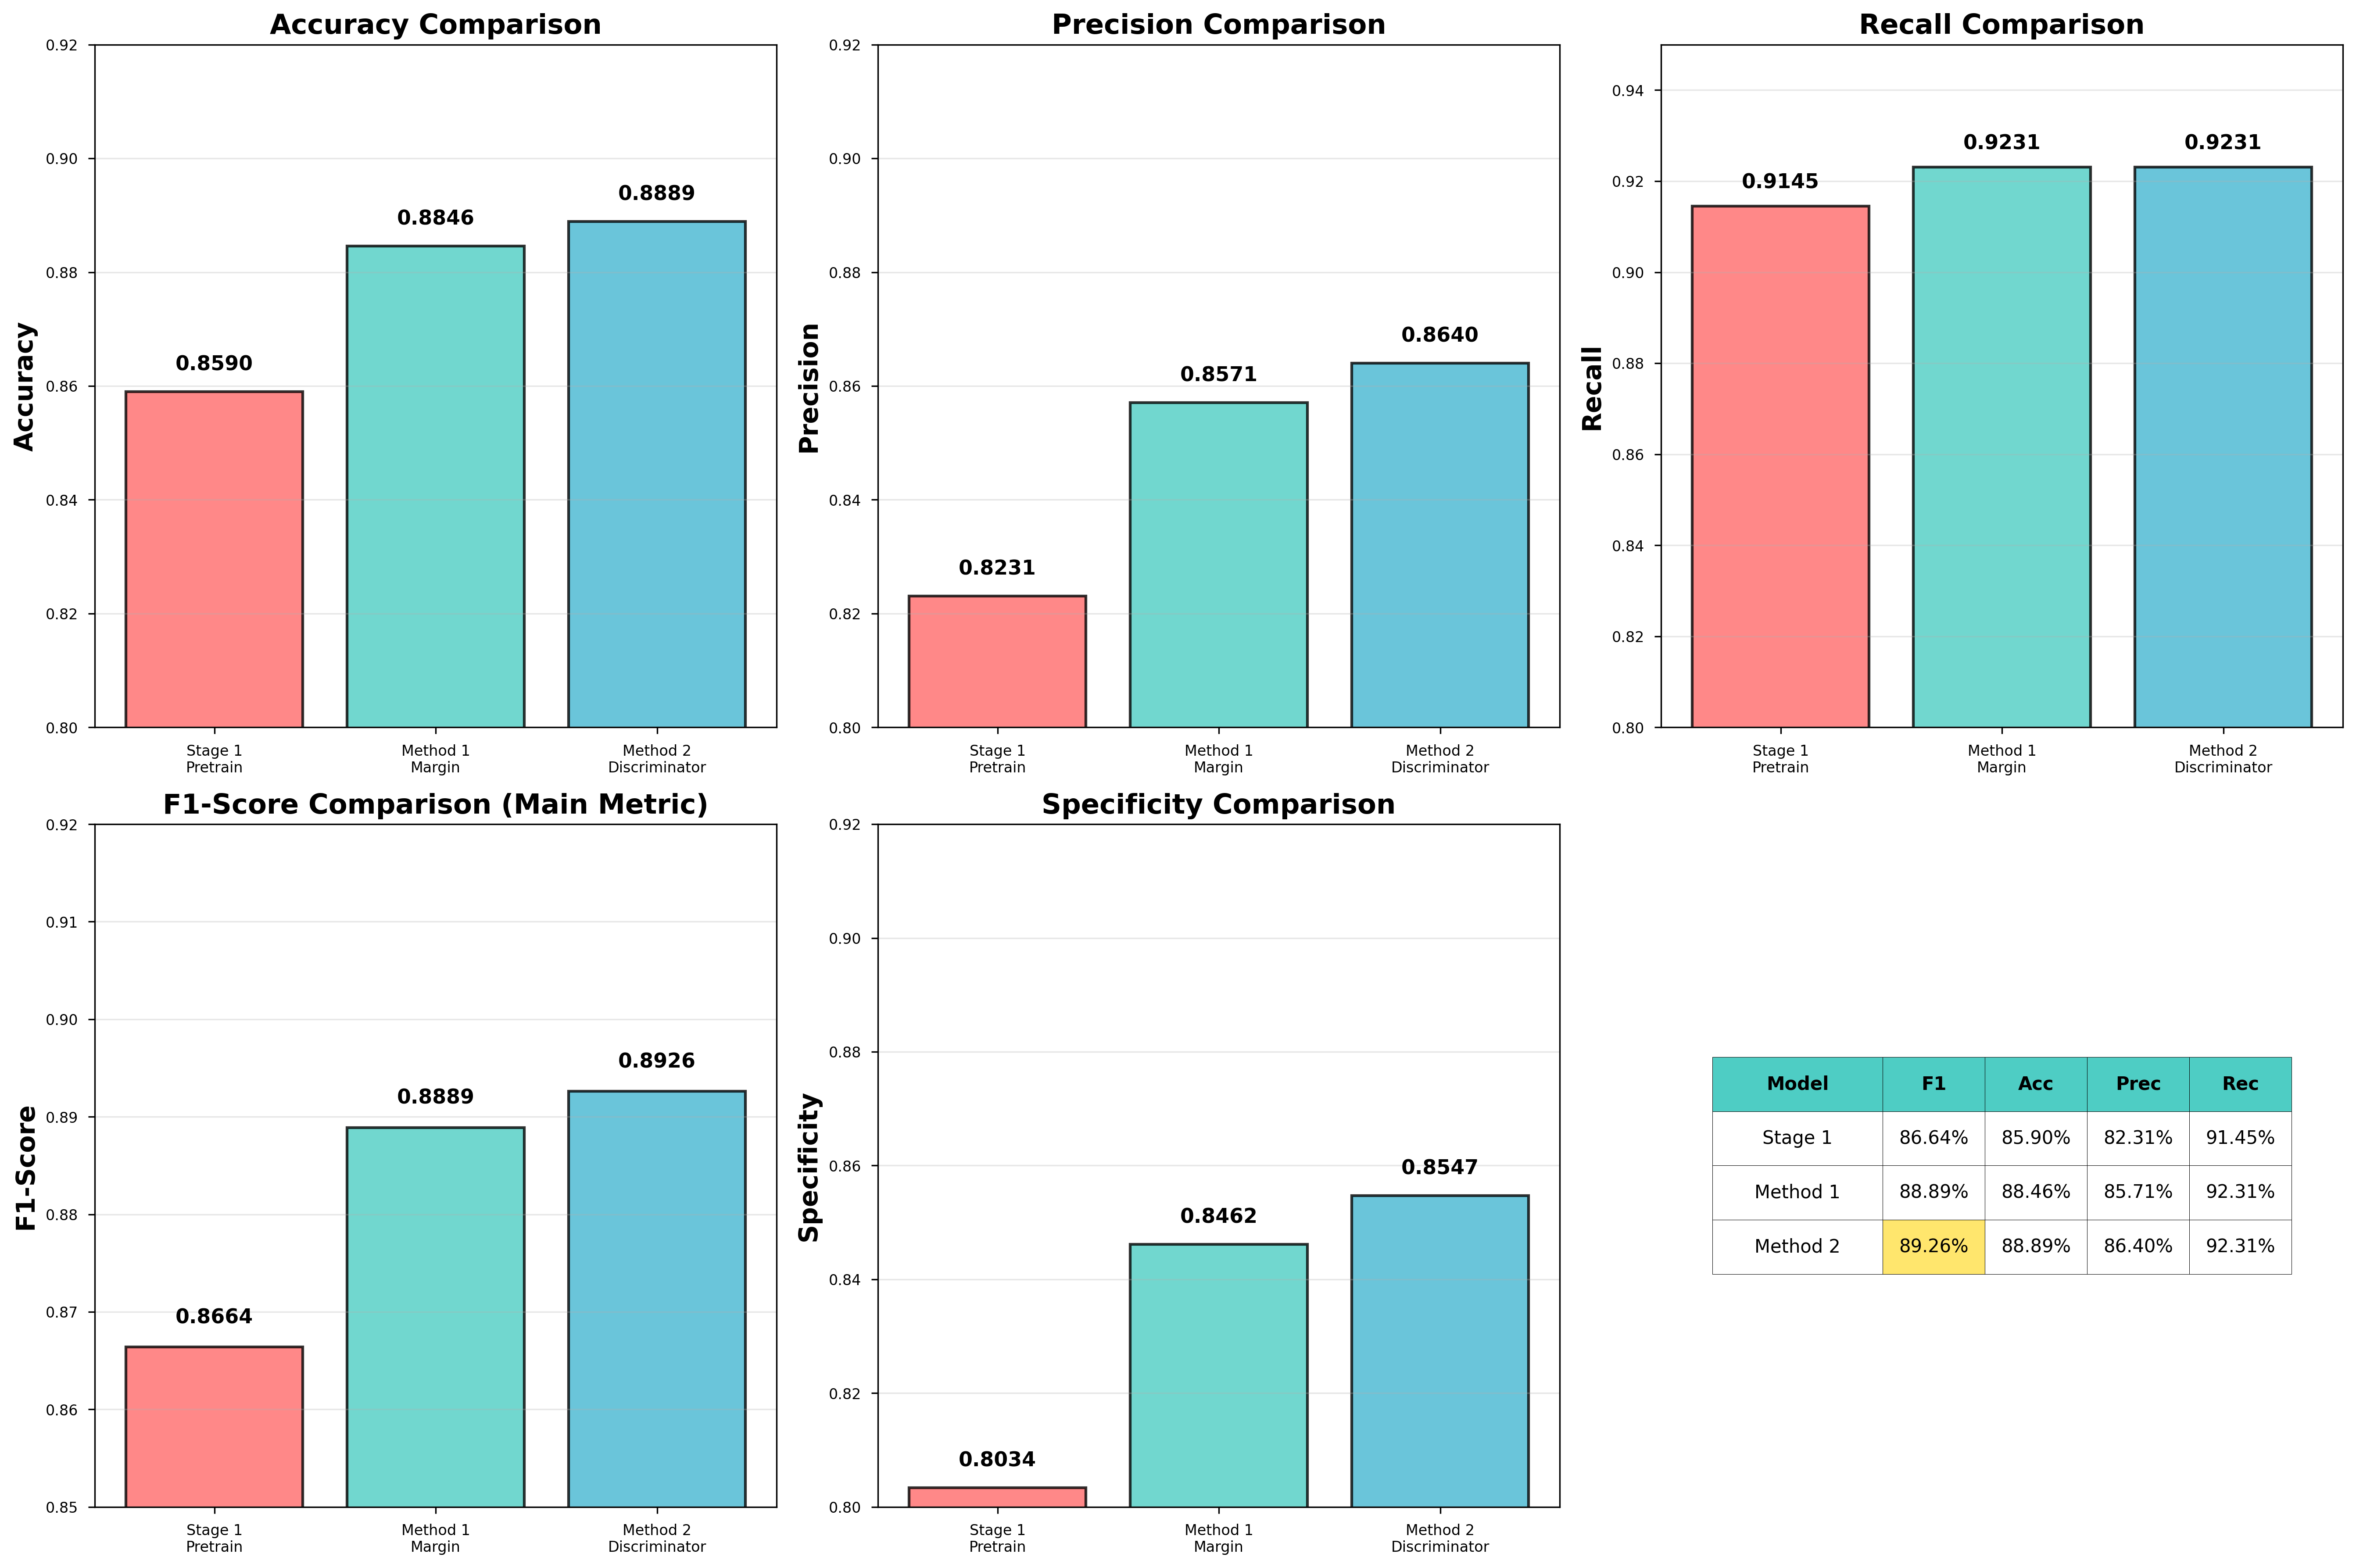
\includegraphics[width=0.48\textwidth]{paper_figures/figure1_main_results.png}
\caption{Performance comparison. Method 2 achieves best F1 (89.26\%), outperforming Method 1 (88.89\%) and Stage 1 (86.64\%).}
\label{fig:main_results}
\vspace{-1em}
\end{figure}

\textbf{Key Observations:}

\textbf{(1) Strong performance with minimal fake data.} Method 2 achieves 89.26\% F1 using only 538 fake samples, validating our hypothesis that extensive fake datasets are unnecessary with proper one-class pretraining.

\textbf{(2) High recall (92.31\%)} indicates models rarely misclassify fakes as real—critical for security where false acceptance is costly.

\textbf{(3) Balanced specificity (84-85\%)} maintains good real acceptance while detecting fakes, avoiding overly conservative rejection.

\textbf{(4) Both Stage 2 methods effective,} with Method 2 slightly superior (+0.37\% F1). Both significantly outperform Stage 1 (+2.25\% and +2.62\% F1).

Figure~\ref{fig:confusion_matrices} shows confusion matrices.

\begin{figure}[t]
\centering
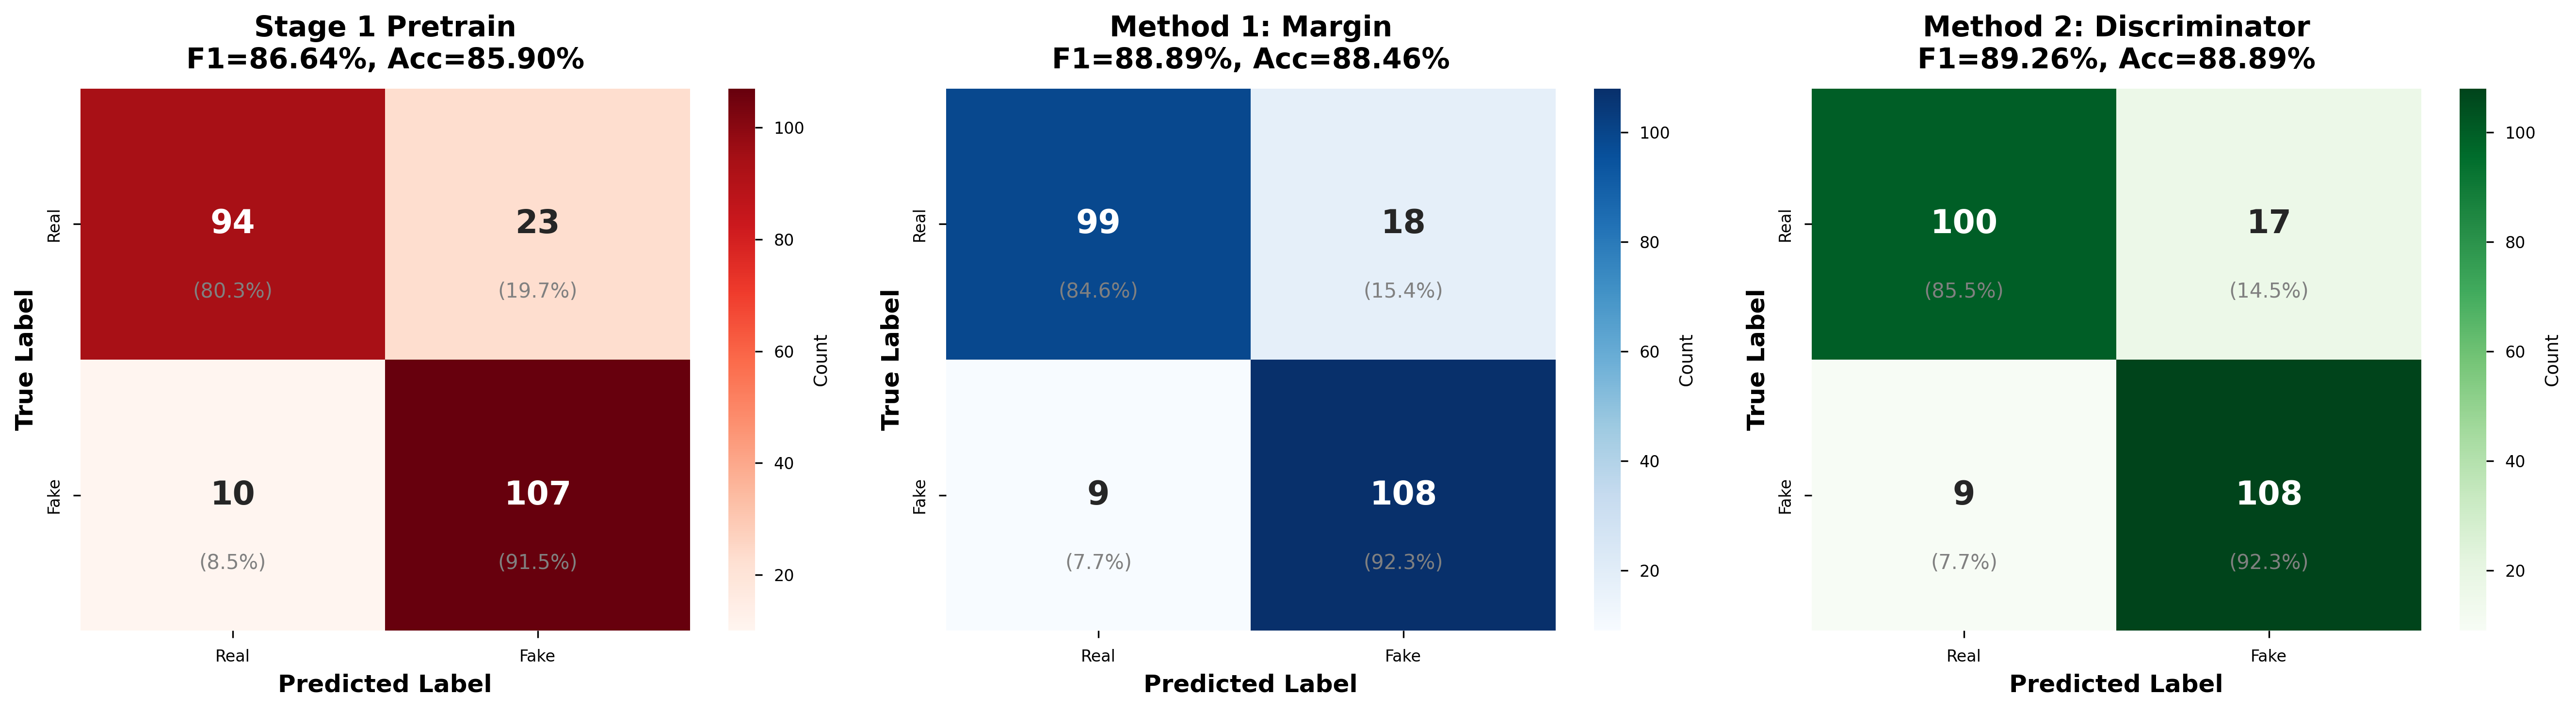
\includegraphics[width=0.48\textwidth]{paper_figures/figure2_confusion_matrices.png}
\caption{Confusion matrices. Method 2: TN=100, FP=17, FN=9, TP=108. Both Stage 2 methods substantially reduce false negatives vs. Stage 1.}
\label{fig:confusion_matrices}
\vspace{-1em}
\end{figure}

\subsection{Frequency Band Analysis}

Frequency decomposition provides interpretability. Reconstruction error analysis reveals fake videos exhibit characteristic patterns:

\begin{itemize}
\itemsep0em
    \item \textbf{LF anomalies:} Unnatural head pose transitions in replay attacks due to camera shake
    \item \textbf{BP anomalies:} Asynchronous lip motion in audio-driven fakes where mouth movements don't match speech frequencies
    \item \textbf{HF anomalies:} Missing micro-expressions in synthetic faces lacking subtle muscle movements
\end{itemize}

This enables forensic analysis: examining which band exhibits strongest anomaly identifies likely attack method, guiding targeted countermeasures.

\subsection{Computational Efficiency}

Our model requires 2.7M parameters, processes 10-second videos in $\sim$50ms on single GPU (RTX 3090). Comparisons:
\begin{itemize}
\itemsep0em
    \item Video-based 3D CNNs: $>$100M parameters, $>$500ms
    \item Transformer methods: $>$80M parameters, $>$300ms
    \item Optical flow: No learned parameters, $>$200ms
\end{itemize}

Landmark-only representation provides $>10\times$ speedup vs. pixel-based methods. Parameter efficiency (38$\times$ smaller) enables deployment on mobile phones and embedded systems.

\section{Discussion}

\subsection{Key Contributions}

\textbf{Landmark efficiency:} Operating on 40 landmarks reduces dimensionality by $>1000\times$ while preserving motion dynamics. This validates that motion patterns, not appearance, are primary signals for liveness detection. Achieving 89.26\% F1 with 2.7M parameters demonstrates motion alone suffices.

\textbf{Data-efficient learning:} Two-stage paradigm addresses fundamental challenge: obtaining diverse fake samples is expensive and outdated quickly. Learning real manifold first via one-class VAE, then fine-tuning with minimal fake data (538 samples), shows extensive fake datasets are unnecessary. Stage 1 provides strong initialization; Stage 2 adds discriminative boundaries with minimal data.

\textbf{Interpretable frequency decomposition:} Band-split architecture inspired by human perception: we process facial motion at different temporal scales (slow head movements, speech-synchronized lip motion, rapid micro-expressions). Explicitly modeling these bands provides interpretability—analysts identify \emph{which} band exhibits anomalies, guiding countermeasure development.

\subsection{Comparison with Prior Work}

Traditional methods like LBP texture analysis require hand-crafted features, struggle with diverse attacks. Deep learning achieves higher accuracy but requires large-scale datasets ($>10,000$ samples), expensive models ($>100$M parameters), full video frames.

Our method achieves competitive performance with modest dataset (1088 real, 538 fake), compact model (2.7M parameters, 38$\times$ smaller), lightweight input (landmarks only, $>1000\times$ reduction), and interpretable architecture.

Key insight: \emph{motion patterns}, not appearance, are primary liveness signals. Focusing on this via landmarks and frequency decomposition achieves efficiency without sacrificing accuracy.

\subsection{Limitations and Future Work}

\textbf{Landmark dependency:} Assumes reliable landmark detection. Extreme poses or occlusions may degrade performance. Future work: incorporate uncertainty estimation or fallback mechanisms.

\textbf{Attack diversity:} Dataset includes replay and audio-driven attacks. Evaluation on emerging threats (diffusion-based deepfakes, adversarial perturbations, 3D masks) needed. Frequency decomposition framework is general and should extend, but empirical validation required.

\textbf{Cross-dataset generalization:} Experiments use single dataset. Cross-dataset evaluation would assess generalization to different devices, lighting, demographics, compression artifacts.

\textbf{Real-time deployment:} While inference is fast (50ms), real-time streaming requires engineering optimizations (batching, INT8 quantization, asynchronous processing).

\subsection{Broader Impact}

Liveness detection is dual-use technology. While enhancing security, we acknowledge potential misuse for unauthorized surveillance or tracking. We advocate transparent deployment with user consent.

The interpretability facilitates bias detection: analysts examine if certain groups consistently fail specific band filters, enabling targeted fairness interventions. We recommend fallback authentication methods (PIN, challenge-response) for inclusive deployment.

\section{Conclusion}

We presented efficient two-stage framework for face liveness detection operating exclusively on facial landmarks. Combining one-class VAE pretraining with minimal discriminative fine-tuning and frequency-decoupled architecture, we achieve 89.26\% F1 with only 2.7M parameters—38$\times$ smaller than video-based approaches.

Results challenge conventional wisdom that liveness detection requires extensive fake datasets and expensive models. With proper inductive biases (landmark motion, frequency decomposition) and learning strategies (one-class pretraining), competitive performance is achievable with minimal resources. Frequency decomposition provides interpretability, revealing characteristic anomalies for various attack types.

Future work will explore cross-dataset generalization, robustness to emerging attacks, and real-time deployment optimizations.

{\small
\bibliographystyle{plain}
\bibliography{references}
}

\end{document}
